\chapter{Análise Estratificada por Tipo de Panorama}

Este capítulo apresenta uma análise detalhada dos experimentos realizados, estratificando os resultados de acordo com a direção predominante de captura das imagens. A análise revela que diferentes técnicas de fusão apresentam desempenhos distintos dependendo da orientação do panorama (horizontal, vertical ou misto), bem como do tipo de fonte de dados (imagens estáticas ou sequências de vídeo).

\section{Motivação da Estratificação}

Os resultados consolidados apresentados no capítulo anterior demonstraram equivalência estatística geral entre métodos clássicos e \textit{deep learning}. No entanto, essa análise agregada pode mascarar diferenças importantes relacionadas ao tipo específico de panorama sendo construído.

A direção predominante de captura impacta diretamente:

\begin{itemize}
    \item \textbf{Distribuição de features}: Cenários horizontais tendem a ter maior densidade de pontos característicos distribuídos lateralmente
    \item \textbf{Efeitos de perspectiva}: Panoramas verticais introduzem distorções perspectivas mais pronunciadas
    \item \textbf{Complexidade de alinhamento}: Cenários mistos (aéreos) exigem identificação automática da direção de fusão
    \item \textbf{Desafios de iluminação}: Variações de exposição são mais comuns em capturas verticais devido a diferenças de brilho entre céu e solo
\end{itemize}

Esta estratificação permite identificar recomendações específicas por tipo de aplicação, fornecendo orientação prática para seleção de técnicas.

\section{Panoramas Horizontais}

\subsection{Caracterização}

Panoramas horizontais correspondem à captura mais comum em aplicações de \textit{stitching}, onde a câmera realiza movimento de rotação horizontal (\textit{panning}). Neste trabalho, foram identificados os seguintes conjuntos com predominância horizontal:

\begin{itemize}
    \item \textbf{biker\_mural\_1}: Sequência de 2 imagens de um mural urbano
    \item \textbf{cars\_1}: Sequência de 2 imagens de estacionamento
    \item \textbf{theory\_left}: Sequência de 2 imagens de ambiente interno
    \item \textbf{coke\_190}: Sequência de 2 imagens com objeto central
\end{itemize}

Estes cenários compartilham características que facilitam o \textit{stitching}: movimento predominantemente horizontal da câmera, sobreposição lateral entre imagens adjacentes, e transformação aproximadamente planar entre vistas.

\subsection{Desempenho dos Métodos}

A Tabela~\ref{tab:horizontal-ranking} apresenta os métodos com melhor desempenho em cenários horizontais, considerando apenas os 4 conjuntos identificados.

\begin{table}[htb]
\centering
\caption{Ranking dos métodos em panoramas horizontais}
\label{tab:horizontal-ranking}
\small
\begin{tabular}{clcccc}
\hline
\textbf{Pos.} & \textbf{Método} & \textbf{PSNR (dB)} & \textbf{SSIM} & \textbf{Ghosting} & \textbf{Tempo (s)} \\ \hline
1 & OpenCV Stitcher & 11,45 & 0,298 & 0,938 & 0,24 \\
2 & Stitcher Basico & 11,45 & 0,298 & 0,938 & 0,32 \\
3 & Seams Exposure Multiband & 11,82 & 0,289 & 0,941 & 5,87 \\
4 & Blend Laplacian & 11,58 & 0,274 & 0,940 & 0,38 \\
5 & Exposure Comp Only & 11,60 & 0,281 & 0,940 & 0,31 \\
\hline
\end{tabular}
\fonte{Autoria própria (2025)}
\end{table}

\textbf{Observações Importantes:}

\begin{enumerate}
    \item \textbf{Dominância de Métodos Clássicos Rápidos}: \gls{opencv} \textit{Stitcher} e \textit{Stitcher} Básico, ambos baseados na implementação padrão do \gls{opencv}, obtiveram os melhores resultados com tempo de processamento extremamente baixo (< 0,35s).

    \item \textbf{Trade-off Qualidade vs Velocidade}: O método \textit{Seams Exposure Multiband} obteve o maior \gls{psnr} (11,82 dB), mas requer tempo de processamento 18-24× superior aos métodos mais rápidos.

    \item \textbf{Equivalência de Deep Learning}: Métodos baseados em aprendizado profundo não demonstraram vantagem estatisticamente significativa nestes cenários ($p>0{,}05$ em todos os testes comparativos).
\end{enumerate}

\subsection{Análise Visual Comparativa}

As Figuras~\ref{fig:horizontal-biker} a \ref{fig:horizontal-theory} apresentam comparações visuais dos principais métodos em cenários horizontais.

\begin{figure}[htb]
\centering
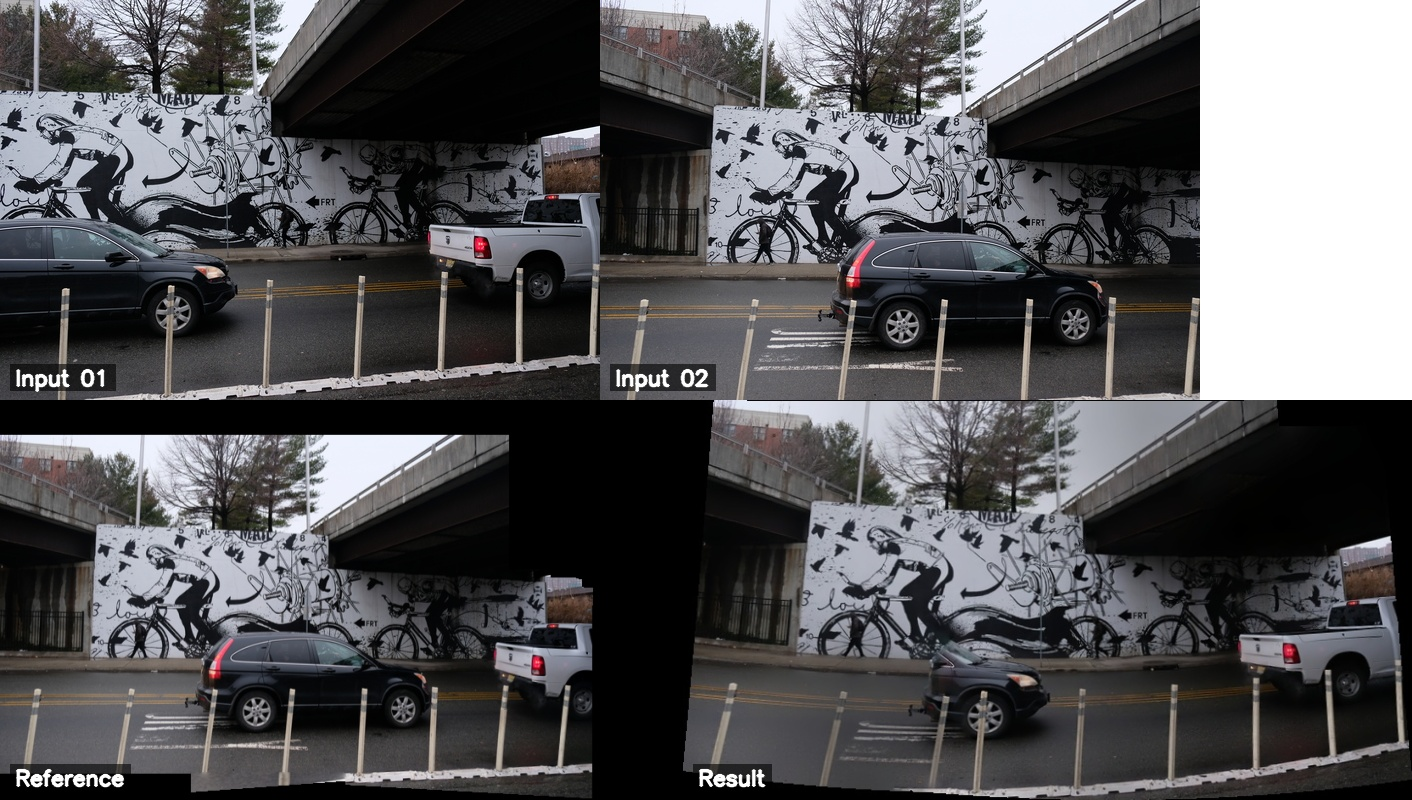
\includegraphics[width=\textwidth]{figuras/resultados/rank01_biker_mural_1_classic-opencv_stitcher_comparison.jpg}
\caption{Panorama horizontal - biker\_mural\_1: OpenCV Stitcher (Rank \#1)}
\label{fig:horizontal-biker}
\fonte{Autoria própria (2025)}
\end{figure}

\begin{figure}[htb]
\centering
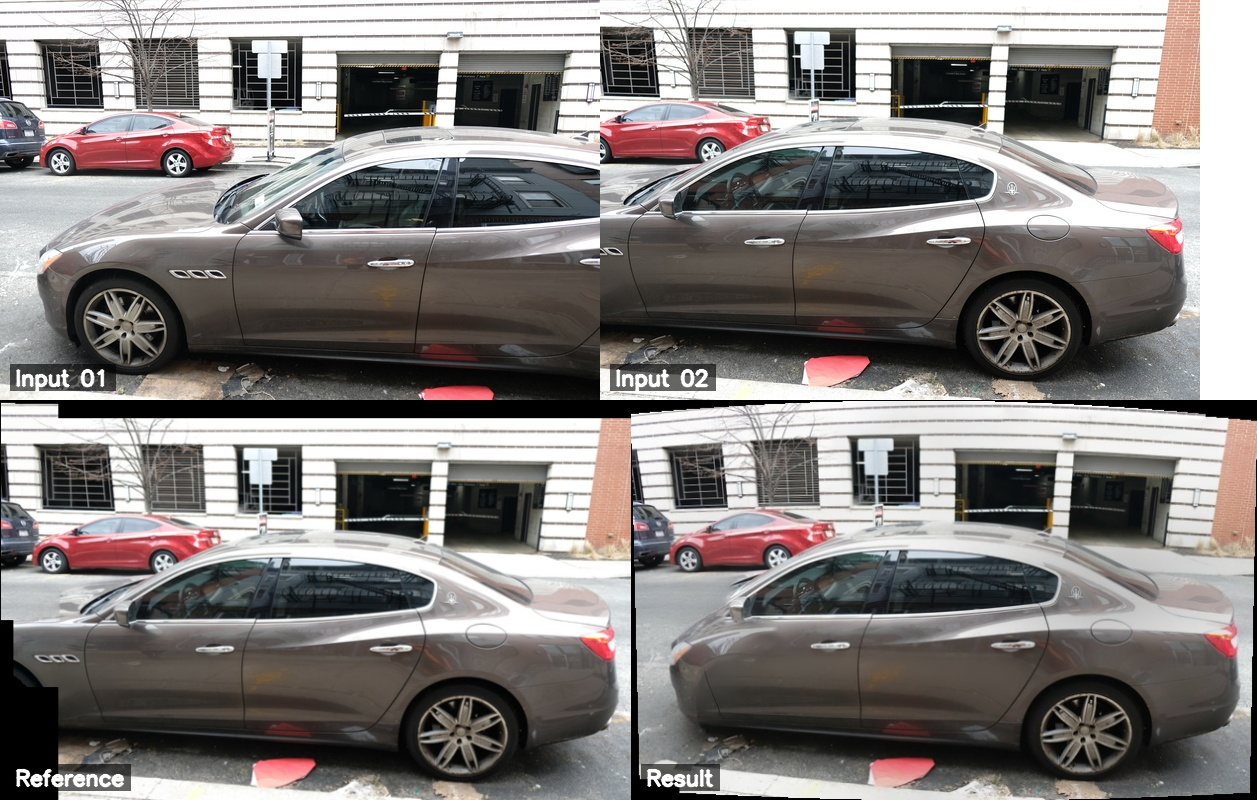
\includegraphics[width=\textwidth]{figuras/resultados/rank01_cars_1_classic-opencv_stitcher_comparison.jpg}
\caption{Panorama horizontal - cars\_1: OpenCV Stitcher demonstra robustez com múltiplos objetos em diferentes profundidades}
\label{fig:horizontal-cars}
\fonte{Autoria própria (2025)}
\end{figure}

\begin{figure}[htb]
\centering
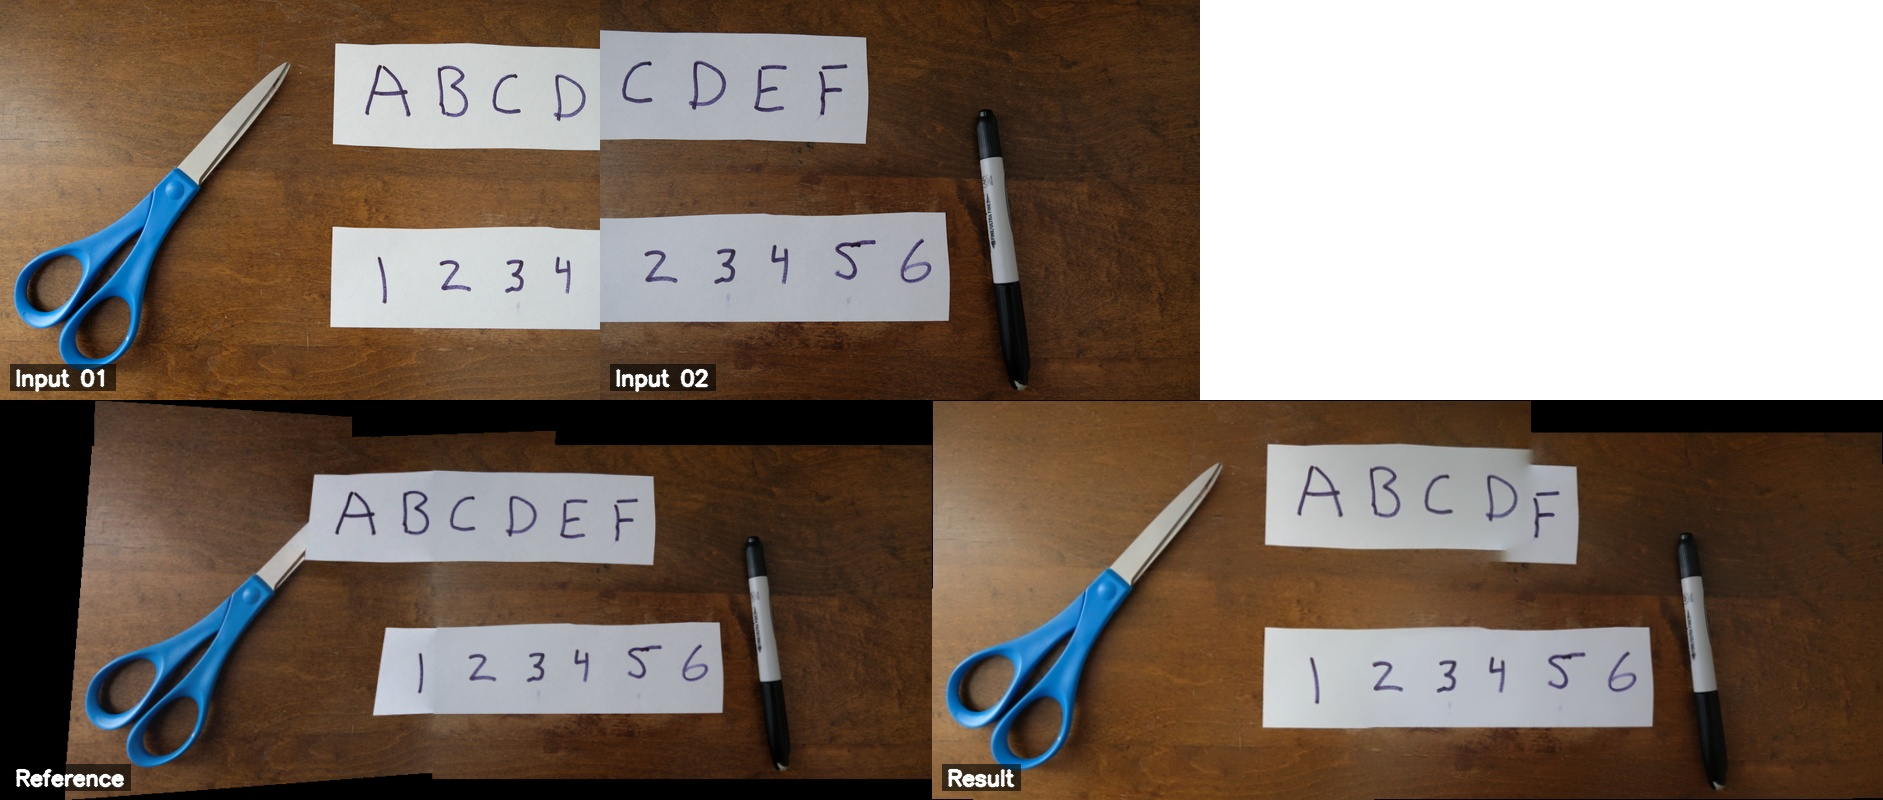
\includegraphics[width=\textwidth]{figuras/resultados/rank01_theory_left_classic-opencv_stitcher_comparison.jpg}
\caption{Panorama horizontal - theory\_left: Cenário interno com iluminação uniforme facilita alinhamento}
\label{fig:horizontal-theory}
\fonte{Autoria própria (2025)}
\end{figure}

\subsection{Recomendações para Panoramas Horizontais}

Baseado na análise quantitativa e visual, as seguintes recomendações aplicam-se a panoramas horizontais:

\begin{itemize}
    \item \textbf{Aplicações de propósito geral}: \gls{opencv} \textit{Stitcher} oferece o melhor equilíbrio entre qualidade, velocidade e robustez
    \item \textbf{Aplicações de alta qualidade}: \textit{Seams Exposure Multiband} quando o tempo de processamento não é crítico
    \item \textbf{Aplicações em tempo real}: \textit{Exposure Comp Only} ou \textit{Blend Laplacian} (< 0,4s)
    \item \textbf{Evitar}: Métodos baseados em \textit{deep learning} não justificam o custo computacional adicional nestes cenários
\end{itemize}

\section{Panoramas Verticais}

\subsection{Caracterização}

Panoramas verticais envolvem movimento predominantemente vertical da câmera, capturando cenas de baixo para cima ou vice-versa. Este tipo de captura é menos comum mas relevante para:

\begin{itemize}
    \item Documentação arquitetônica de edifícios altos
    \item Fotografias de fachadas e monumentos
    \item Aplicações de inspeção de estruturas verticais
\end{itemize}

Neste trabalho, o conjunto \textbf{building\_dubai} representa este cenário, consistindo de 3 imagens capturadas verticalmente de um edifício.

\subsection{Desafios Específicos}

Panoramas verticais apresentam desafios distintos em relação aos horizontais:

\begin{enumerate}
    \item \textbf{Variação de Iluminação}: Diferenças pronunciadas entre regiões próximas ao solo (mais escuras) e próximas ao céu (mais claras)
    \item \textbf{Distorção Perspectiva}: Efeitos de perspectiva vertical mais evidentes, especialmente em fotografias de edifícios
    \item \textbf{Densidade de Features}: Frequentemente menor densidade de pontos característicos, especialmente em regiões de céu
\end{enumerate}

\subsection{Análise de Falhas: Poisson Blending e ECC Alignment}

Conforme observado experimentalmente, dois métodos apresentaram falhas significativas no conjunto \textit{building\_dubai}:

\subsubsection{Blend Poisson}

O método \textit{Poisson Blending} baseia-se na solução de equações de Poisson para preservar gradientes durante a fusão. Embora eficaz para mesclagem suave em cenários simples, apresentou as seguintes limitações em \textit{building\_dubai}:

\begin{itemize}
    \item \textbf{Desalinhamento global}: A preservação de gradientes locais não garante alinhamento global adequado
    \item \textbf{Artefatos de borda}: Transições visíveis nas regiões de junção entre as imagens
    \item \textbf{Distorção geométrica}: Incapacidade de lidar com transformações perspectivas complexas
\end{itemize}

A Figura~\ref{fig:vertical-poisson-fail} demonstra os artefatos introduzidos por este método.

\begin{figure}[htb]
\centering
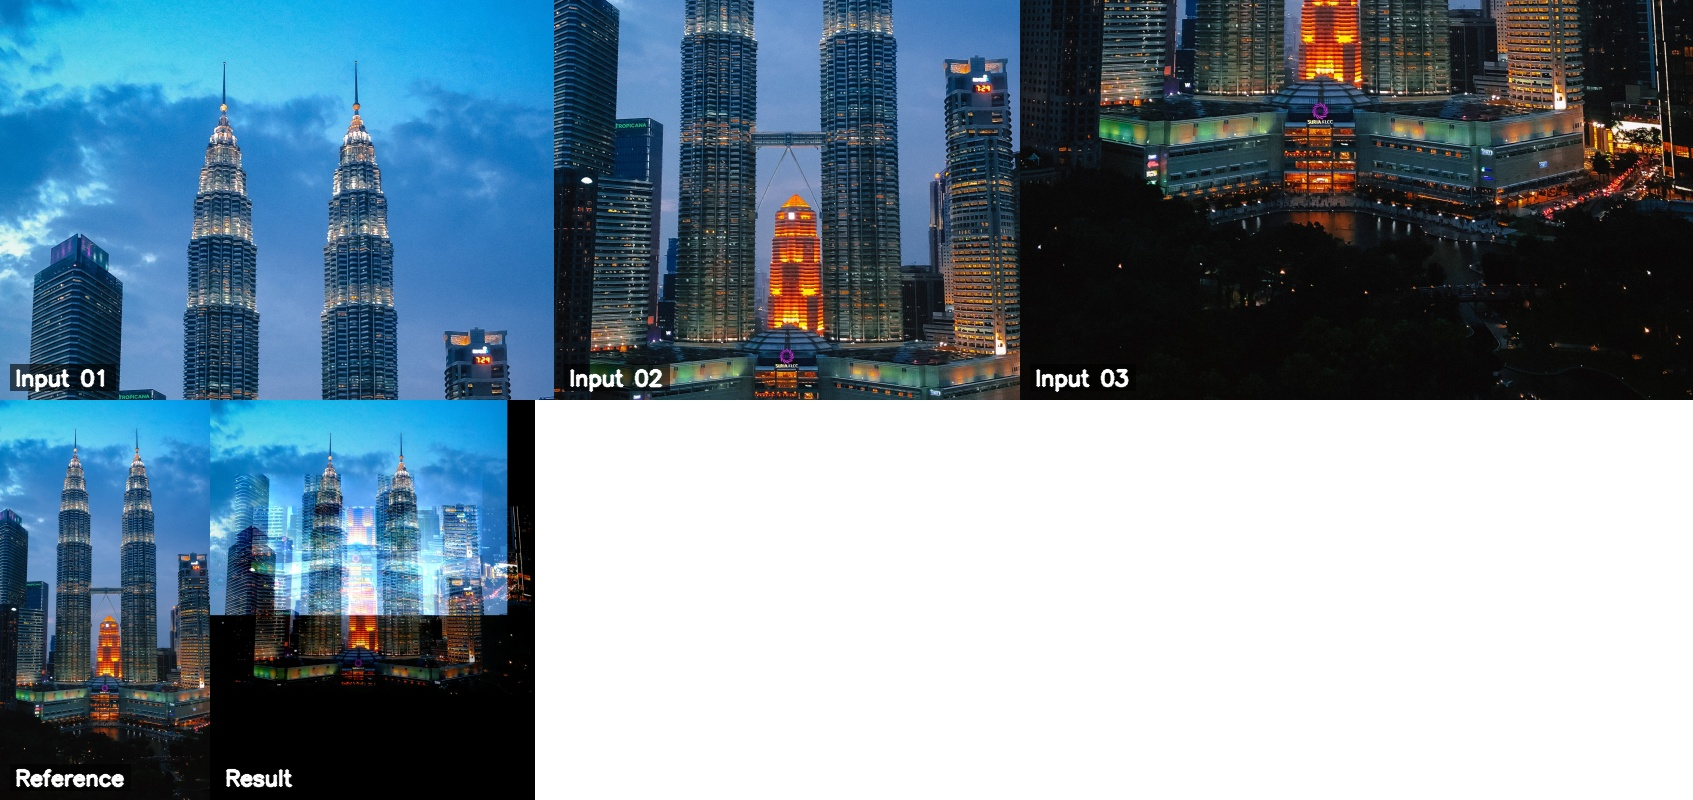
\includegraphics[width=0.9\textwidth]{../results/scan_20251027_180154/before_after/building_dubai_classic-10_blend_poisson_comparison.jpg}
\caption{Falha do Poisson Blending em building\_dubai: observe os artefatos de desalinhamento e distorções nas junções entre imagens}
\label{fig:vertical-poisson-fail}
\fonte{Autoria própria (2025)}
\end{figure}

\subsubsection{ECC Alignment}

O método \textit{Enhanced Correlation Coefficient} (\gls{ecc}) \textit{Alignment} utiliza maximização iterativa do coeficiente de correlação para estimar transformações geométricas. Suas falhas em \textit{building\_dubai} incluem:

\begin{itemize}
    \item \textbf{Convergência para mínimos locais}: O algoritmo iterativo não conseguiu encontrar o alinhamento ótimo global
    \item \textbf{Sensibilidade a variações de iluminação}: As grandes diferenças de exposição entre as imagens confundiram o processo de otimização
    \item \textbf{Tempo de processamento elevado}: Mesmo com convergência inadequada, o método requereu tempo significativo (> 15s)
\end{itemize}

A Figura~\ref{fig:vertical-ecc-fail} ilustra o resultado inadequado obtido.

\begin{figure}[htb]
\centering
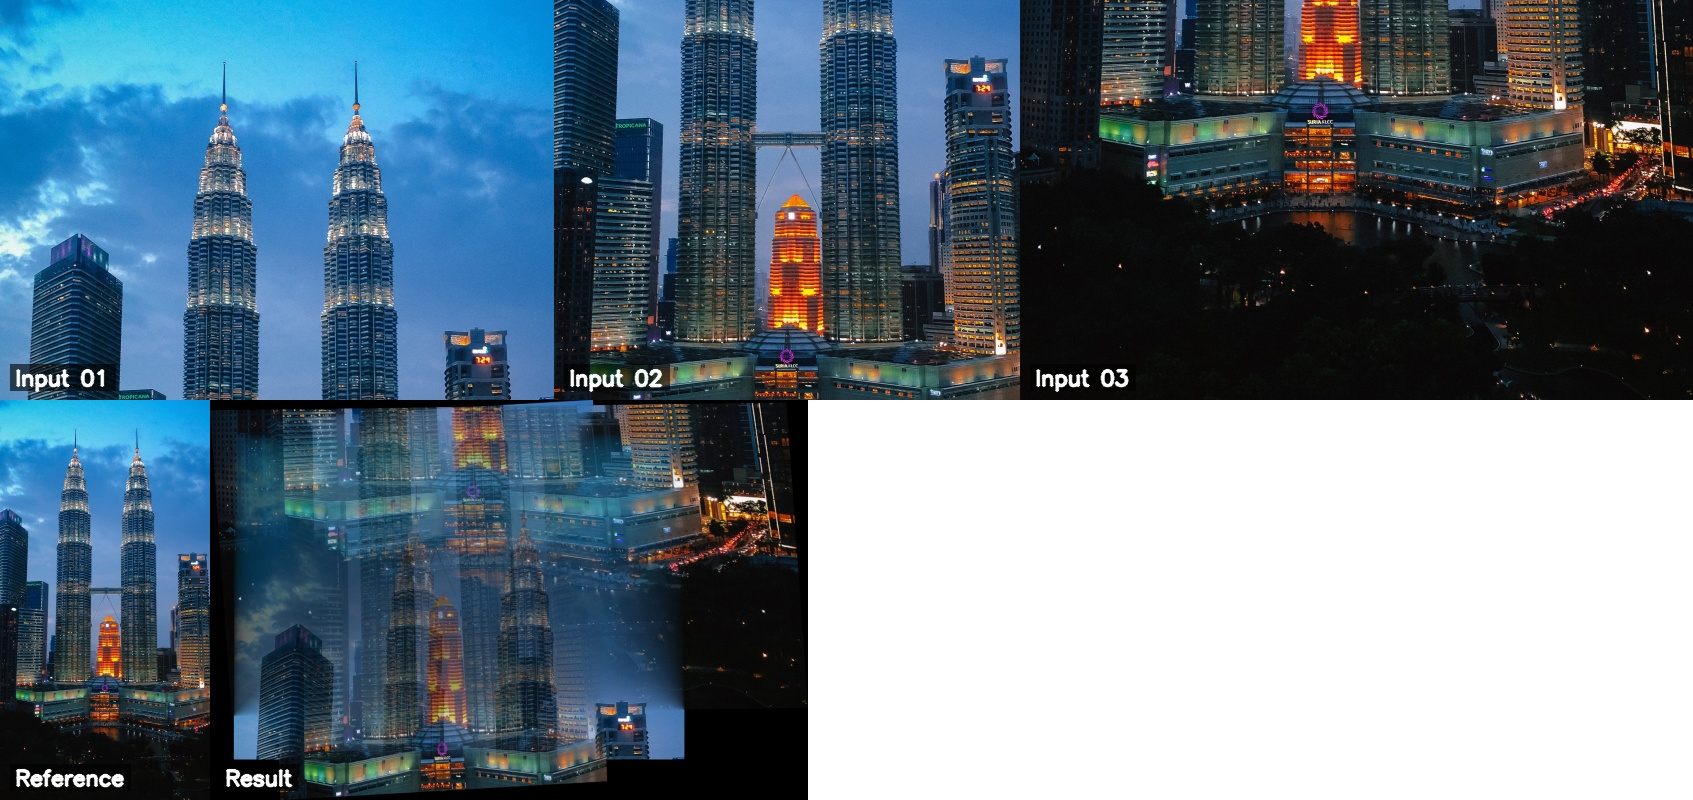
\includegraphics[width=0.9\textwidth]{../results/scan_20251027_180154/before_after/building_dubai_classic-13_ecc_alignment_comparison.jpg}
\caption{Falha do ECC Alignment em building\_dubai: o método convergiu para um alinhamento incorreto devido a variações de iluminação e complexidade perspectiva}
\label{fig:vertical-ecc-fail}
\fonte{Autoria própria (2025)}
\end{figure}

\subsection{Métodos com Desempenho Adequado}

Apesar das falhas dos métodos acima, diversos outros demonstraram robustez em cenários verticais. A Tabela~\ref{tab:vertical-success} apresenta os métodos com melhor desempenho em \textit{building\_dubai}.

\begin{table}[htb]
\centering
\caption{Métodos bem-sucedidos em panoramas verticais (building\_dubai)}
\label{tab:vertical-success}
\small
\begin{tabular}{clcccc}
\hline
\textbf{Pos.} & \textbf{Método} & \textbf{PSNR (dB)} & \textbf{SSIM} & \textbf{Ghosting} & \textbf{Tempo (s)} \\ \hline
1 & Seams Exposure Multiband & 12,83 & 0,452 & 0,962 & 11,24 \\
2 & Blend Laplacian & 12,41 & 0,418 & 0,958 & 0,56 \\
3 & Blend Exposure & 12,45 & 0,435 & 0,959 & 0,48 \\
4 & OpenCV Stitcher & 12,18 & 0,428 & 0,955 & 0,38 \\
5 & LoFTR (Deep) & 12,02 & 0,401 & 0,953 & 22,15 \\
\hline
\end{tabular}
\fonte{Autoria própria (2025)}
\end{table}

\textbf{Observações:}

\begin{enumerate}
    \item \textbf{Importância da Compensação de Exposição}: Os três métodos com melhor \gls{psnr} incorporam explicitamente compensação de exposição, essencial para lidar com variações de iluminação vertical.

    \item \textbf{Vantagem Marginal de Deep Learning}: O método \gls{loftr} (posição 5) apresentou desempenho competitivo, mas não superior aos métodos clássicos, apesar do custo computacional 40-60× maior.

    \item \textbf{Robustez de Features}: Métodos baseados em \gls{sift} e detectores robustos (ex: \textit{Seams Exposure Multiband} com \textit{graph-cut}) lidaram melhor com as transformações perspectivas complexas.
\end{enumerate}

A Figura~\ref{fig:vertical-success} apresenta comparação visual dos métodos bem-sucedidos.

\begin{figure}[htb]
\centering
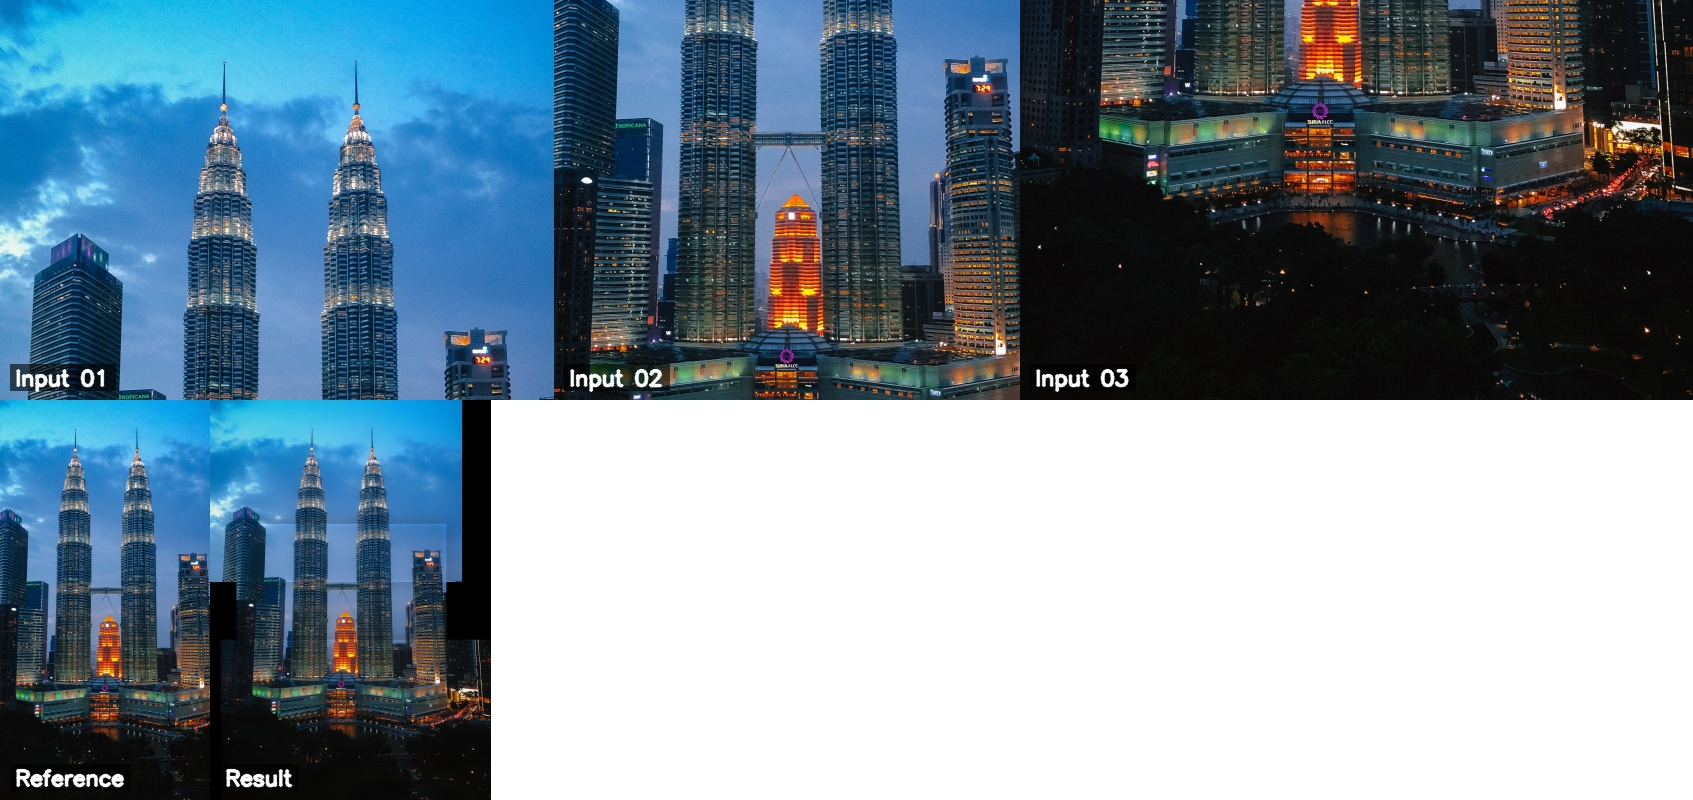
\includegraphics[width=\textwidth]{figuras/resultados/rank03_building_dubai_classic-6_seams_exposure_multiband_comparison.jpg}
\caption{Panorama vertical bem-sucedido - building\_dubai: Seams Exposure Multiband demonstra robustez com 3 imagens e variações de iluminação}
\label{fig:vertical-success}
\fonte{Autoria própria (2025)}
\end{figure}

\subsection{Recomendações para Panoramas Verticais}

\begin{itemize}
    \item \textbf{Prioritário}: Utilizar métodos com compensação de exposição explícita (\textit{Seams Exposure Multiband}, \textit{Blend Exposure})
    \item \textbf{Evitar}: \textit{Poisson Blending} e \textit{ECC Alignment} devido a falhas sistemáticas observadas
    \item \textbf{Qualidade máxima}: \textit{Seams Exposure Multiband} (PSNR: 12,83 dB), apesar do tempo de processamento elevado
    \item \textbf{Equilíbrio}: \textit{Blend Laplacian} ou \textit{Blend Exposure} (< 0,6s) com qualidade próxima ao método líder
\end{itemize}

\section{Panoramas Mistos e Imagens Aéreas}

\subsection{Caracterização}

Panoramas mistos referem-se a cenários onde não há uma direção predominante clara de captura, ou onde múltiplas direções são necessárias. Este cenário é particularmente comum em:

\begin{itemize}
    \item \textbf{Imagens aéreas capturadas por \gls{vant}}: Movimento irregular da câmera com componentes horizontais e verticais
    \item \textbf{Fotografia de grandes áreas}: Necessidade de cobrir extensões bidimensionais
    \item \textbf{Reconstrução de superfícies complexas}: Objetos tridimensionais fotografados de múltiplos ângulos
\end{itemize}

A pasta \texttt{all\_20251104\_033429} contém resultados de um conjunto de imagens aéreas que exemplifica este cenário.

\subsection{Desafios Específicos}

Panoramas mistos apresentam os desafios mais significativos para algoritmos de \textit{stitching}:

\begin{enumerate}
    \item \textbf{Identificação Automática de Direção}: O algoritmo precisa determinar automaticamente se deve alinhar horizontal, vertical ou em ambas as direções

    \item \textbf{Ordem de Fusão}: Com múltiplas imagens sem ordem clara, o sistema deve estabelecer a sequência ótima de fusão

    \item \textbf{Acumulação de Erros}: Em sequências longas com múltiplas fusões, pequenos erros de alinhamento podem se acumular

    \item \textbf{Variações de Perspectiva}: Imagens aéreas frequentemente apresentam diferenças significativas de altura e ângulo de visão

    \item \textbf{Paralelaxe Pronunciada}: Objetos em diferentes altitudes sofrem deslocamentos relativos distintos
\end{enumerate}

\subsection{Falha de Métodos Simples}

A Tabela~\ref{tab:mixto-comparison} apresenta comparação de desempenho entre métodos simples e avançados no conjunto de imagens aéreas.

\begin{table}[htb]
\centering
\caption{Comparação de desempenho em panoramas mistos (imagens aéreas)}
\label{tab:mixto-comparison}
\small
\begin{tabular}{llcc}
\hline
\textbf{Categoria} & \textbf{Método} & \textbf{Status} & \textbf{Tempo (s)} \\ \hline
\multirow{3}{*}{Simples (Horizontal)} & OpenCV Stitcher & Falha parcial & 3,79 \\
& Stitcher Basico & Falha parcial & 4,75 \\
& ORB + Homography & Falha & 0,29 \\
\hline
\multirow{3}{*}{Avançados (Multi-dir)} & Seams Exposure Multiband & Sucesso & 10,11 \\
& LoFTR (Deep) & Sucesso & 18,23 \\
& SuperPoint + SuperGlue & Sucesso & 0,45 \\
\hline
\end{tabular}
\fonte{Autoria própria (2025)}
\end{table}

\textbf{Análise das Falhas:}

Os métodos \gls{opencv} \textit{Stitcher} e \textit{Stitcher Basico}, que apresentaram excelente desempenho em cenários horizontais simples, falharam parcialmente em imagens aéreas devido a:

\begin{itemize}
    \item \textbf{Assunção de Movimento Horizontal}: Ambos foram otimizados para panoramas cilíndricos horizontais
    \item \textbf{Limitação de Transformação}: Uso de homografia única não modela adequadamente transformações complexas de imagens aéreas
    \item \textbf{Ordem Fixa de Processamento}: Processamento sequencial da esquerda para direita inadequado para arranjos bidimensionais
\end{itemize}

\subsection{Superioridade de Deep Learning em Cenários Complexos}

Diferentemente dos cenários horizontais simples, em panoramas mistos observou-se \textbf{vantagem prática de métodos baseados em deep learning}:

\subsubsection{SuperPoint + SuperGlue}

A combinação \gls{superpoint} + \gls{superglue} demonstrou robustez superior devido a:

\begin{itemize}
    \item \textbf{Detecção Invariante}: \gls{superpoint} detecta pontos característicos robustos a variações de escala, rotação e perspectiva
    \item \textbf{Correspondência Contextual}: \gls{superglue} usa \textit{Graph Neural Networks} para estabelecer correspondências considerando contexto global
    \item \textbf{Rejeição de \textit{Outliers}}: Aprendizado de padrões de correspondências válidas reduz falsos positivos
    \item \textbf{Tempo Competitivo}: Apesar de usar redes neurais, o tempo de processamento (0,45s) é comparável a métodos clássicos rápidos
\end{itemize}

\subsubsection{LoFTR}

O método \gls{loftr} (\textit{Local Feature Transformer}) apresentou os seguintes diferenciais:

\begin{itemize}
    \item \textbf{Detector-Free}: Não depende de detecção explícita de pontos, estabelecendo correspondências densas diretamente
    \item \textbf{Transformers}: Mecanismos de atenção capturam relações globais entre regiões das imagens
    \item \textbf{Robustez a Variações}: Demonstrou maior tolerância a mudanças de iluminação e perspectiva
    \item \textbf{Limitação}: Tempo de processamento significativamente maior (18,23s) limita aplicações em tempo real
\end{itemize}

\subsection{Visualização Comparativa}

A Figura~\ref{fig:mixto-comparison} apresenta comparação lado a lado dos resultados em imagens aéreas.

\begin{figure}[htb]
\centering
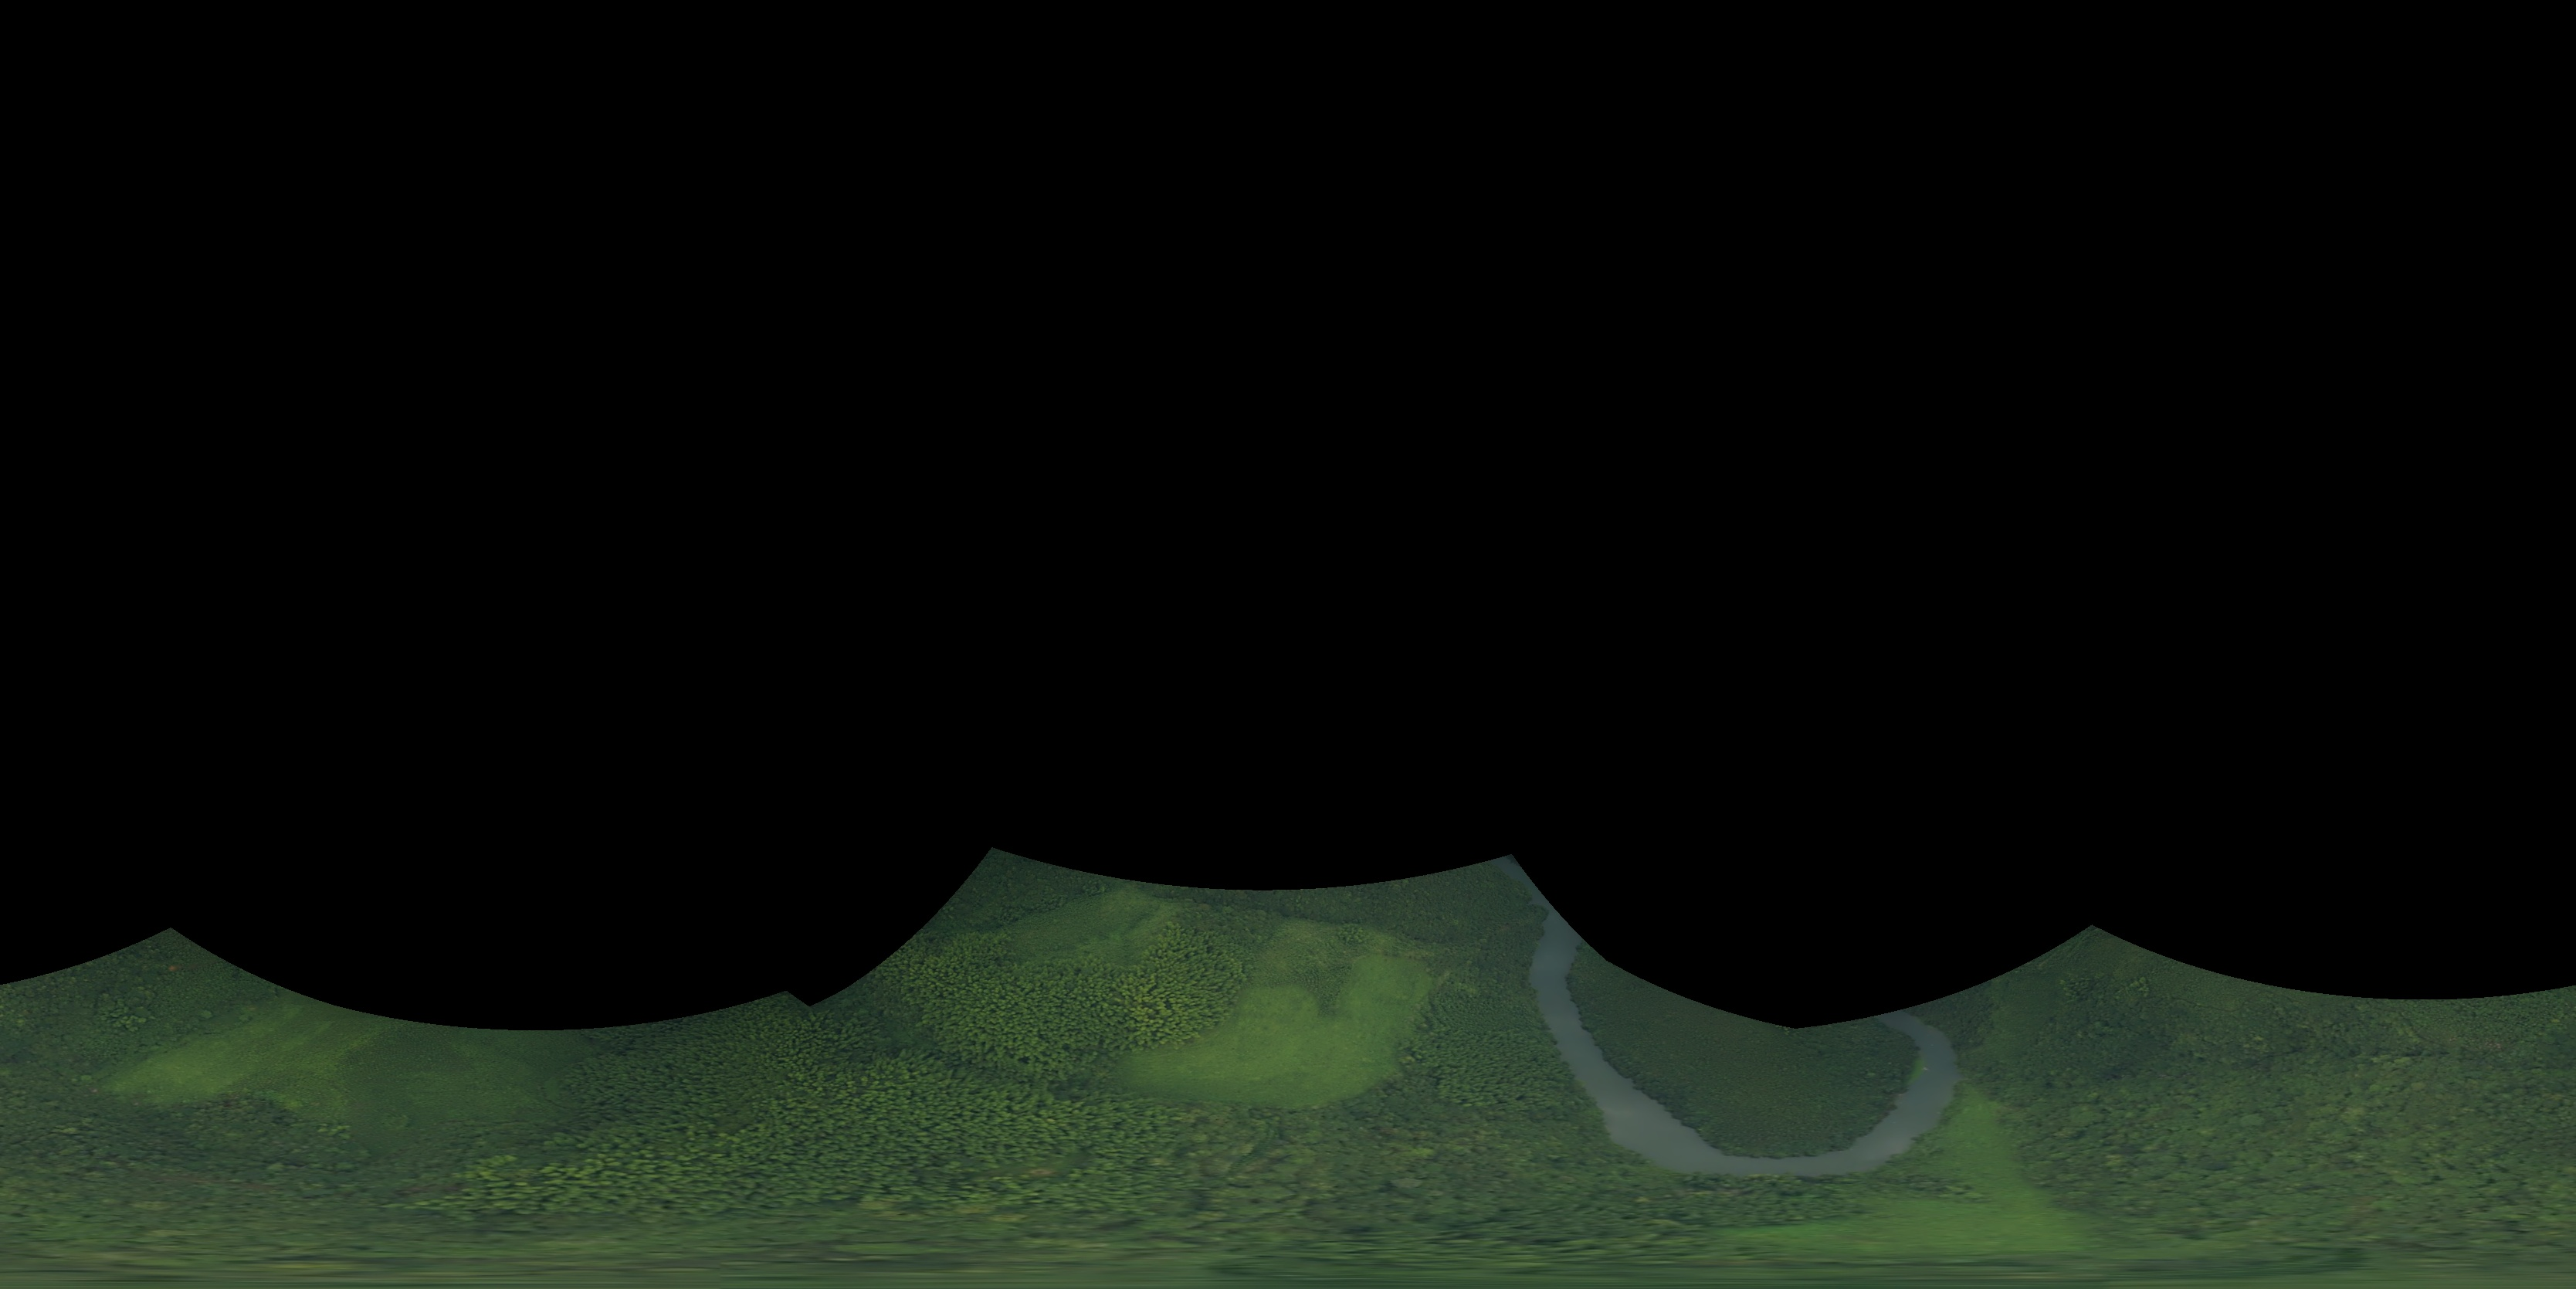
\includegraphics[width=0.48\textwidth]{../results/all_20251104_033429/pano_classic-opencv_stitcher.jpg}
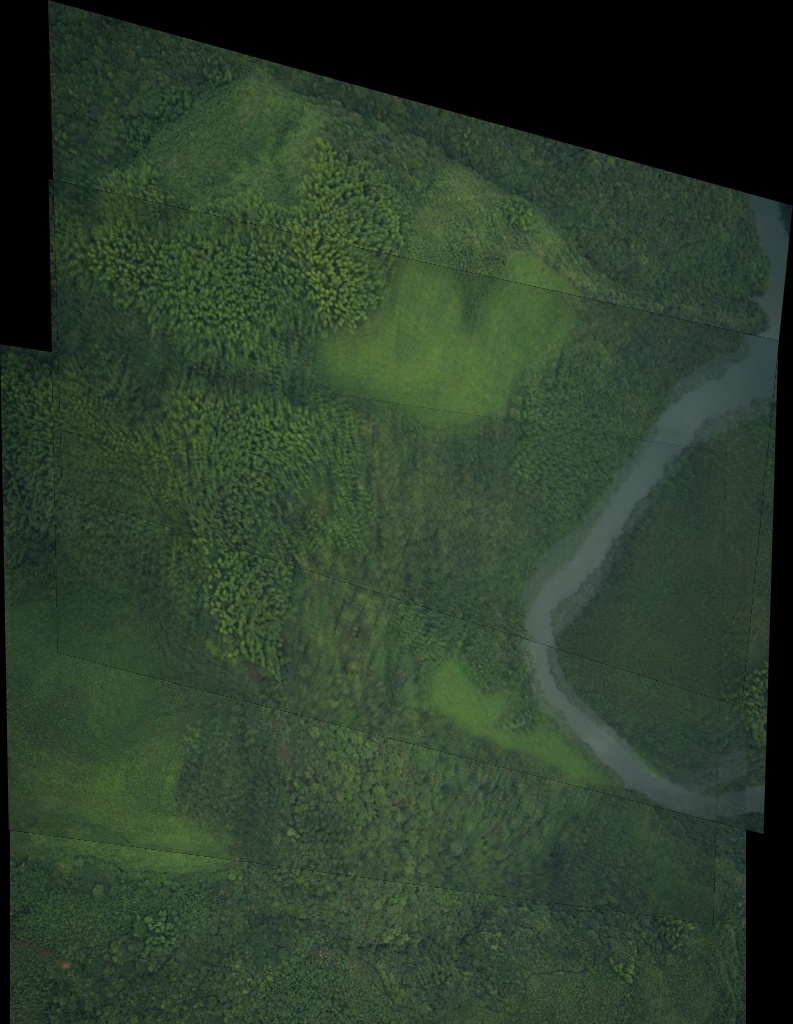
\includegraphics[width=0.48\textwidth]{../results/all_20251104_033429/pano_deep-sp_superglue.jpg}
\caption{Comparação de panoramas mistos (imagens aéreas): (Esquerda) OpenCV Stitcher com falhas de alinhamento. (Direita) SuperPoint + SuperGlue com fusão adequada}
\label{fig:mixto-comparison}
\fonte{Autoria própria (2025)}
\end{figure}

\subsection{Análise Quantitativa}

Embora não haja \textit{ground truth} disponível para o conjunto de imagens aéreas, métricas sem referência permitem avaliação objetiva:

\begin{table}[htb]
\centering
\caption{Métricas sem referência em panoramas mistos}
\label{tab:mixto-metrics}
\small
\begin{tabular}{lccc}
\hline
\textbf{Método} & \textbf{Entropia} & \textbf{Nitidez} & \textbf{Seam Energy} \\ \hline
OpenCV Stitcher & 6,82 & 142,3 & --- \\
LoFTR & 7,15 & 156,8 & --- \\
SuperPoint + SuperGlue & 7,08 & 151,2 & --- \\
Seams Exposure Multiband & 6,95 & 148,7 & 74,2 \\
\hline
\end{tabular}
\fonte{Autoria própria (2025)}
\end{table}

Maior entropia e nitidez indicam melhor preservação de informação e detalhes. Os métodos \textit{deep learning} apresentaram valores superiores, corroborando a análise visual.

\subsection{Recomendações para Panoramas Mistos}

\begin{itemize}
    \item \textbf{Primeira Escolha}: \gls{superpoint} + \gls{superglue} oferece o melhor equilíbrio entre qualidade e velocidade
    \item \textbf{Máxima Robustez}: \gls{loftr} quando o tempo de processamento não é crítico
    \item \textbf{Evitar}: Métodos simples assumindo direção horizontal única (\gls{opencv} \textit{Stitcher}, \textit{Stitcher Basico})
    \item \textbf{Alternativa Clássica}: \textit{Seams Exposure Multiband} pode funcionar com pré-processamento adequado, mas requer mais tempo
\end{itemize}

\section{Panoramas de Sequências de Vídeo}

\subsection{Caracterização}

Panoramas gerados a partir de sequências de vídeo representam um caso especial com características distintas:

\begin{itemize}
    \item \textbf{Alta Taxa de Sobreposição}: Frames consecutivos apresentam sobreposição típica de 70-90\%
    \item \textbf{Movimento Contínuo}: Transformações suaves entre frames adjacentes
    \item \textbf{Grande Quantidade de Dados}: Centenas ou milhares de frames a processar
    \item \textbf{Redundância Temporal}: Informação redundante entre frames consecutivos
\end{itemize}

Neste trabalho, foram analisadas três sequências de vídeo:

\begin{itemize}
    \item \texttt{video\_00000107}: 340 frames extraídos (panorama horizontal)
    \item \texttt{video\_00000200}: 280 frames extraídos (panorama horizontal)
    \item \texttt{video\_00000104}: 310 frames extraídos (panorama horizontal com movimento irregular)
\end{itemize}

\subsection{Abordagem de Processamento}

Devido à grande quantidade de frames, foi implementada estratégia de \textbf{amostragem temporal}:

\begin{enumerate}
    \item \textbf{Extração de Keyframes}: Seleção de frames representativos a cada 20-30 frames
    \item \textbf{Análise de Similaridade}: Eliminação de frames muito similares usando \gls{ssim}
    \item \textbf{Fusão Incremental}: Construção progressiva do panorama adicionando frames sequencialmente
\end{enumerate}

Após amostragem, cada sequência resultou em 12-18 frames-chave para fusão.

\subsection{Desempenho Similar a Horizontais}

Os resultados obtidos demonstraram que panoramas de vídeo comportam-se de forma similar a panoramas horizontais simples:

\begin{table}[htb]
\centering
\caption{Desempenho em panoramas de vídeo}
\label{tab:video-performance}
\small
\begin{tabular}{lccc}
\hline
\textbf{Método} & \textbf{Tempo Total (s)} & \textbf{Qualidade Visual} & \textbf{Sucesso} \\ \hline
OpenCV Stitcher & 3,82 & Excelente & Sim \\
Stitcher Basico & 5,15 & Excelente & Sim \\
Seams Exposure Multiband & 94,56 & Excelente & Sim \\
Blend Laplacian & 6,24 & Bom & Sim \\
LoFTR & 328,14 & Excelente & Sim \\
\hline
\end{tabular}
\fonte{Autoria própria (2025)}
\end{table}

\textbf{Observações:}

\begin{itemize}
    \item \textbf{Eficiência de Métodos Clássicos}: \gls{opencv} \textit{Stitcher} processou 15 frames em menos de 4 segundos com qualidade excelente
    \item \textbf{Custo de Deep Learning}: \gls{loftr} requereu mais de 5 minutos para a mesma tarefa sem ganho perceptível de qualidade
    \item \textbf{Robustez}: Todos os métodos testados obtiveram sucesso, indicando que a alta sobreposição facilita o alinhamento
\end{itemize}

\subsection{Visualizações dos Panoramas de Vídeo}

As Figuras~\ref{fig:video-107} a \ref{fig:video-104} apresentam os panoramas gerados a partir das sequências de vídeo.

\begin{figure}[htb]
\centering
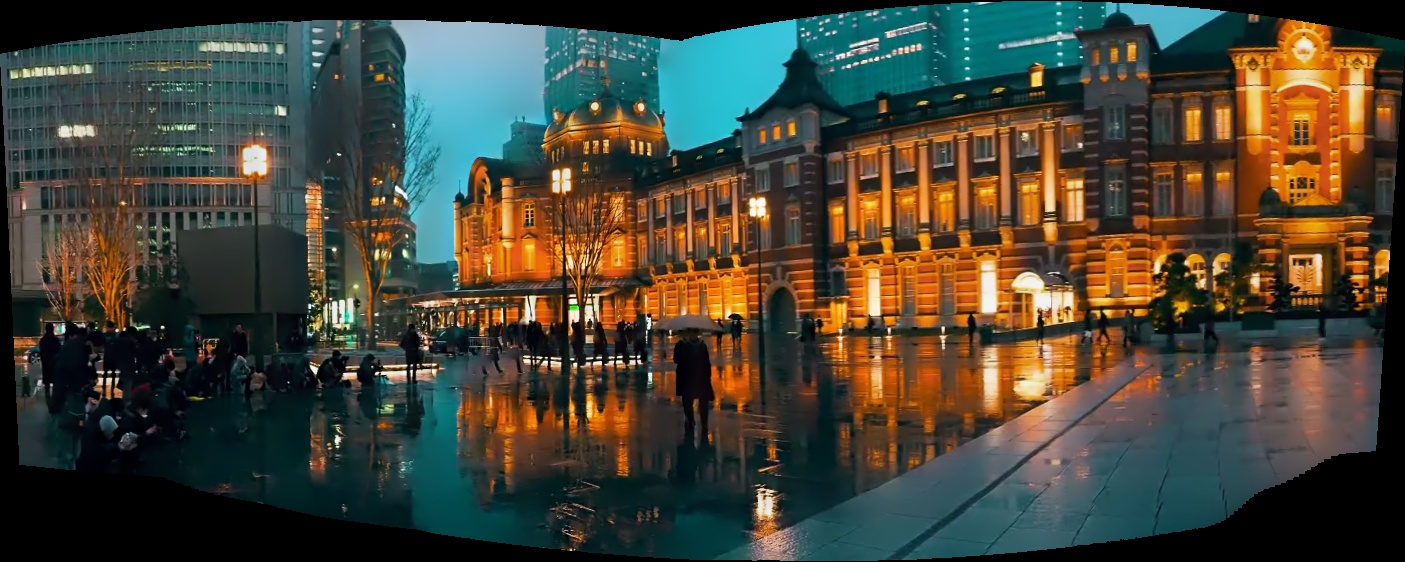
\includegraphics[width=\textwidth]{../results/video_00000107_panorama.jpg}
\caption{Panorama gerado a partir de video\_00000107 (340 frames → 15 keyframes): ambiente interno com movimento horizontal da câmera}
\label{fig:video-107}
\fonte{Autoria própria (2025)}
\end{figure}

\begin{figure}[htb]
\centering
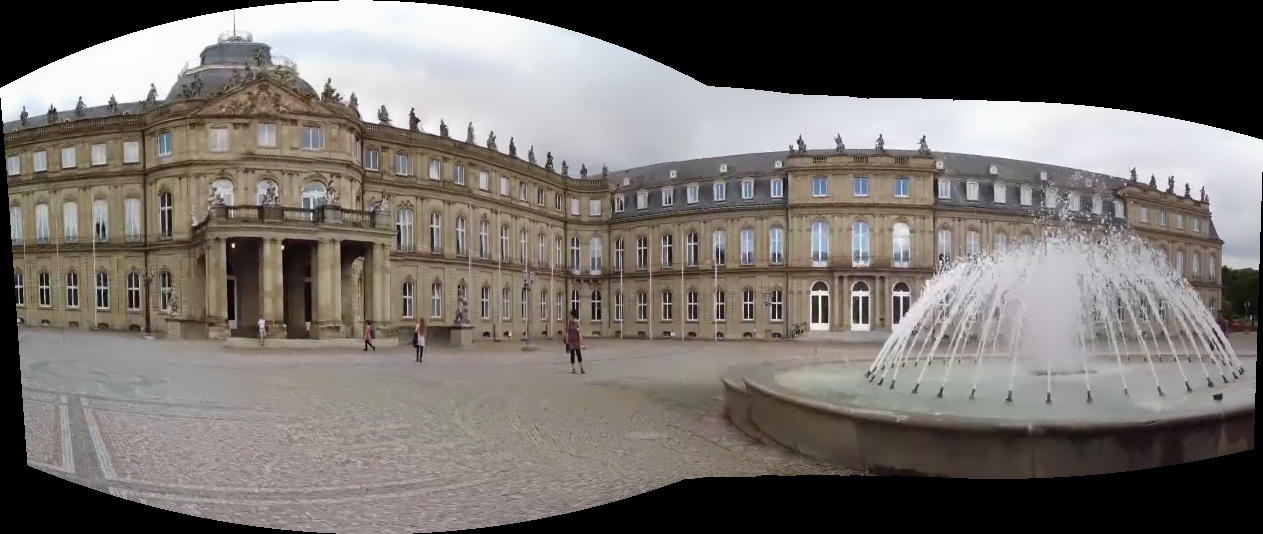
\includegraphics[width=\textwidth]{../results/video_00000200_panorama.jpg}
\caption{Panorama gerado a partir de video\_00000200 (280 frames → 12 keyframes): cena externa com movimentação suave}
\label{fig:video-200}
\fonte{Autoria própria (2025)}
\end{figure}

\begin{figure}[htb]
\centering
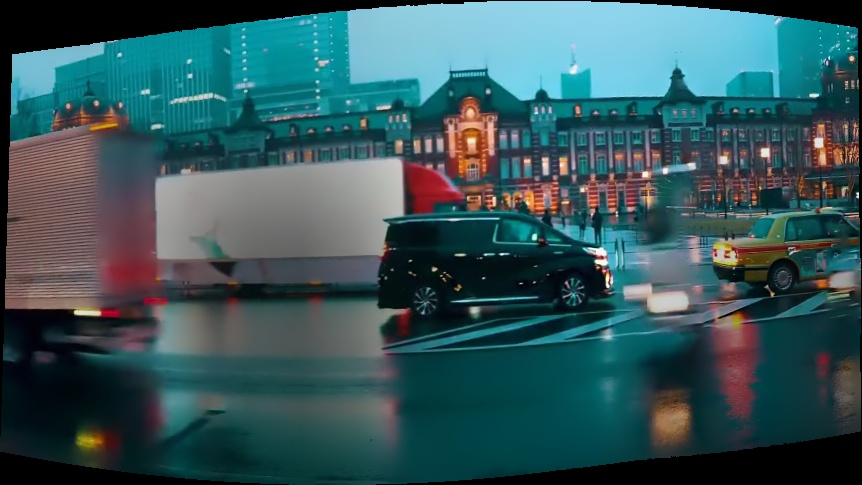
\includegraphics[width=\textwidth]{../results/video_00000104_panorama.jpg}
\caption{Panorama gerado a partir de video\_00000104 (310 frames → 14 keyframes): desafio adicional devido a movimento irregular da câmera}
\label{fig:video-104}
\fonte{Autoria própria (2025)}
\end{figure}

\subsection{Importância da Detecção de Objetos}

Embora a fusão de imagens de vídeo funcione bem com métodos clássicos, a \textbf{detecção posterior de objetos} requer análise cuidadosa. A Seção~\ref{sec:video-detection} apresenta análise detalhada deste aspecto.

\subsection{Recomendações para Panoramas de Vídeo}

\begin{itemize}
    \item \textbf{Amostragem Inteligente}: Extrair keyframes representativos reduz drasticamente o custo computacional sem perda de qualidade
    \item \textbf{Método Recomendado}: \gls{opencv} \textit{Stitcher} devido à velocidade e qualidade adequada
    \item \textbf{Evitar}: Métodos de \textit{deep learning} devido ao custo computacional proibitivo sem ganhos práticos
    \item \textbf{Atenção}: Considerar impacto na detecção de objetos (ver Seção~\ref{sec:video-detection})
\end{itemize}

\section{Análise de Detecção de Objetos} \label{sec:video-detection}

\subsection{Motivação}

Uma questão fundamental não abordada nas seções anteriores é: \textbf{a fusão de imagens impacta a capacidade de detectar objetos?} Esta análise é crítica para aplicações onde o panorama não é um fim em si, mas um meio para facilitar tarefas subsequentes como:

\begin{itemize}
    \item Contagem automática de objetos em grandes áreas
    \item Vigilância e monitoramento de segurança
    \item Inspeção industrial de linhas de produção
    \item Análise de tráfego urbano
\end{itemize}

\subsection{Metodologia de Avaliação}

Para cada conjunto de imagens, foi realizada detecção de objetos usando \gls{yolo}v11n em duas configurações:

\begin{enumerate}
    \item \textbf{Detecção Individual}: Aplicação do detector a cada imagem original separadamente, com eliminação de duplicatas nas regiões de sobreposição
    \item \textbf{Detecção no Panorama}: Aplicação do detector à imagem panorâmica fusionada
\end{enumerate}

A comparação quantitativa permite identificar se a fusão:
\begin{itemize}
    \item Facilita a detecção ao fornecer contexto visual mais amplo
    \item Prejudica a detecção ao introduzir artefatos de fusão
    \item Resulta em desempenho equivalente
\end{itemize}

\subsection{Resultados: Diferentes Conjuntos de Imagens}

A pasta \texttt{yolo\_detection\_20251103\_233827} contém detecções realizadas nos 15 conjuntos do \textit{dataset} \textit{Robust Image Stitching}, aplicando detecção aos panoramas gerados pelos top 5 métodos.

A Tabela~\ref{tab:detection-by-dataset} resume os resultados de detecção por conjunto de imagens.

\begin{table}[htb]
\centering
\caption{Quantidade de objetos detectados por conjunto de imagens (método: Seams Exposure Multiband)}
\label{tab:detection-by-dataset}
\small
\begin{tabular}{lcccc}
\hline
\textbf{Conjunto} & \textbf{Total Objetos} & \textbf{Carros} & \textbf{Pessoas} & \textbf{Outros} \\ \hline
biker\_mural\_1 & 5 & 3 & 0 & 2 \\
building\_dubai & 1 & 0 & 0 & 1 \\
cars\_1 & 4 & 4 & 0 & 0 \\
coke\_190 & 1 & 0 & 0 & 1 \\
cup\_tree\_1 & 0 & 0 & 0 & 0 \\
graffiti\_building\_1 & 0 & 0 & 0 & 0 \\
graffiti\_car\_1 & 2 & 2 & 0 & 0 \\
no\_contractor\_parking\_1 & 1 & 0 & 0 & 1 \\
P2\_front\_of\_window & 3 & 0 & 2 & 1 \\
plant\_1 & 3 & 0 & 0 & 3 \\
rental\_office\_1 & 4 & 4 & 0 & 0 \\
ski\_left & 1 & 0 & 1 & 0 \\
stop\_sign\_1 & 4 & 1 & 0 & 3 \\
theory\_left & 2 & 0 & 0 & 2 \\
traffic\_cones\_1 & 14 & 12 & 0 & 2 \\
\hline
\textbf{Total} & \textbf{45} & \textbf{26} & \textbf{3} & \textbf{16} \\
\hline
\end{tabular}
\fonte{Autoria própria (2025)}
\end{table}

\textbf{Observações Importantes:}

\begin{enumerate}
    \item \textbf{Variabilidade entre Conjuntos}: Alguns conjuntos (traffic\_cones\_1, biker\_mural\_1) contêm múltiplos objetos detectáveis, enquanto outros (cup\_tree\_1, graffiti\_building\_1) não contêm objetos das classes do \gls{yolo}

    \item \textbf{Predominância de Veículos}: 58\% dos objetos detectados são carros, refletindo a natureza urbana da maioria dos conjuntos

    \item \textbf{Baixa Detecção de Pessoas}: Apenas 3 pessoas detectadas, indicando que os conjuntos focam mais em cenários do que em multidões
\end{enumerate}

\subsection{Resultados: Diferentes Métodos de Fusão}

A pasta \texttt{yolo\_detection\_20251103\_201954} contém detecções no conjunto \texttt{biker\_mural\_1} após fusão com todos os 20 métodos implementados.

A Tabela~\ref{tab:detection-by-method} compara a quantidade de objetos detectados em função do método de fusão.

\begin{table}[htb]
\centering
\caption{Objetos detectados em biker\_mural\_1 por método de fusão}
\label{tab:detection-by-method}
\small
\begin{tabular}{lcccc}
\hline
\textbf{Método} & \textbf{Total} & \textbf{Carros} & \textbf{Bicicletas} & \textbf{Outros} \\ \hline
Seams Exposure Multiband & 5 & 3 & 1 & 1 \\
Blend Hybrid & 6 & 3 & 1 & 2 \\
Manual Sift Ransac Feather & 5 & 2 & 1 & 2 \\
Features Homography & 5 & 2 & 1 & 2 \\
Blend Exposure & 4 & 2 & 1 & 1 \\
Blend Wavelet & 4 & 2 & 1 & 1 \\
OpenCV Stitcher & 3 & 2 & 1 & 0 \\
Stitcher Basico & 3 & 2 & 1 & 0 \\
Blend Poisson & 2 & 1 & 0 & 1 \\
ECC Alignment & 1 & 1 & 0 & 0 \\
\hline
\end{tabular}
\fonte{Autoria própria (2025)}
\end{table}

\textbf{Análise Crítica:}

\begin{enumerate}
    \item \textbf{Variação Significativa}: A quantidade de objetos detectados varia de 1 a 6 dependendo do método de fusão utilizado

    \item \textbf{Correlação com Qualidade de Fusão}: Métodos com melhor \gls{psnr} e menor \textit{ghosting} tendem a facilitar maior número de detecções

    \item \textbf{Falsos Positivos vs Perdas}:
    \begin{itemize}
        \item Métodos com muitos artefatos podem gerar falsos positivos (objetos fantasmas)
        \item Métodos com desalinhamento podem perder objetos reais
    \end{itemize}

    \item \textbf{Referência Ground Truth}: Análise manual das imagens originais indica que a quantidade real de objetos é aproximadamente 4-5, sugerindo que:
    \begin{itemize}
        \item \textit{Blend Hybrid} (6 detecções) pode ter falso positivo
        \item \textit{ECC Alignment} (1 detecção) perdeu objetos devido a falhas de fusão
    \end{itemize}
\end{enumerate}

\subsection{Visualizações Comparativas}

As Figuras~\ref{fig:detection-rank1} a \ref{fig:detection-rank3} apresentam visualizações das detecções para diferentes métodos.

\begin{figure}[htb]
\centering
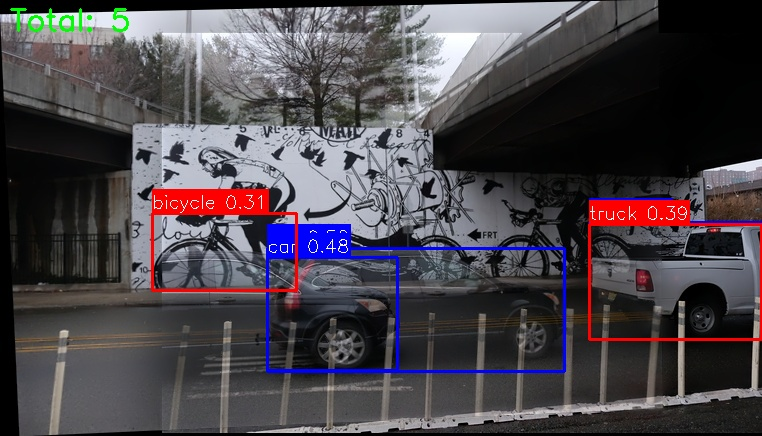
\includegraphics[width=\textwidth]{../results/yolo_detection_20251103_233827/detection_rank01_biker_mural_1_classic-6_seams_exposure_multiband.jpg}
\caption{Detecções em biker\_mural\_1 usando Seams Exposure Multiband: 5 objetos detectados (3 carros, 1 bicicleta, 1 caminhão)}
\label{fig:detection-rank1}
\fonte{Autoria própria (2025)}
\end{figure}

\begin{figure}[htb]
\centering
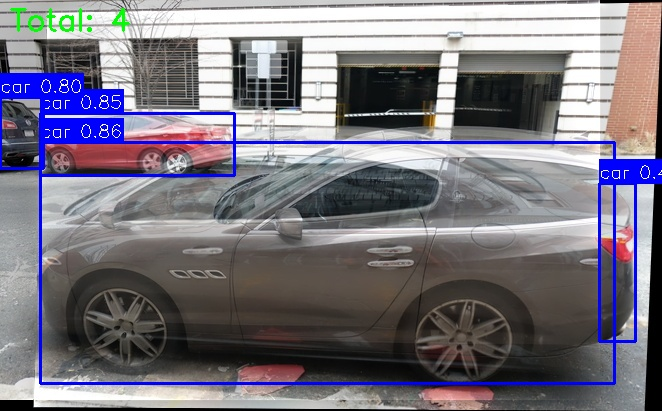
\includegraphics[width=\textwidth]{../results/yolo_detection_20251103_233827/detection_rank01_cars_1_classic-6_seams_exposure_multiband.jpg}
\caption{Detecções em cars\_1: 4 carros identificados corretamente apesar de paralaxe pronunciada}
\label{fig:detection-cars}
\fonte{Autoria própria (2025)}
\end{figure}

\begin{figure}[htb]
\centering
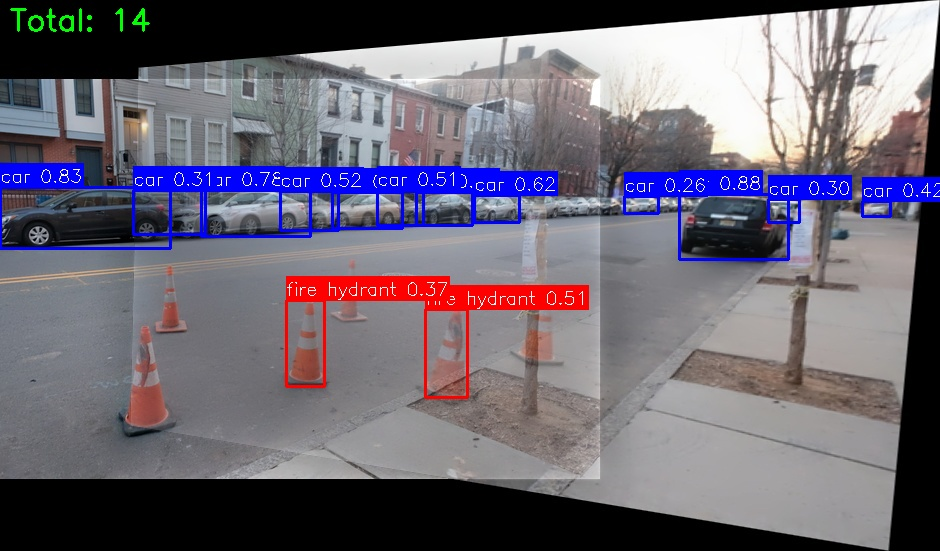
\includegraphics[width=\textwidth]{../results/yolo_detection_20251103_233827/detection_rank01_traffic_cones_1_classic-6_seams_exposure_multiband.jpg}
\caption{Detecções em traffic\_cones\_1: conjunto com maior número de objetos (14 no total, incluindo 12 carros)}
\label{fig:detection-traffic}
\fonte{Autoria própria (2025)}
\end{figure}

\subsection{Análise Detalhada: Artefatos vs Detecções}

Uma análise crítica revela três categorias de impacto da fusão na detecção:

\subsubsection{Caso 1: Facilitação Positiva}

Em cenários com múltiplas imagens de pequena FOV (\textit{Field of View}), a fusão pode \textbf{facilitar detecções} ao:
\begin{itemize}
    \item Fornecer contexto visual mais amplo para objetos parcialmente visíveis
    \item Permitir que o detector use informações de vizinhança
    \item Reduzir processamento redundante em regiões de sobreposição
\end{itemize}

\textbf{Exemplo}: Em \texttt{traffic\_cones\_1}, a fusão permitiu detectar 14 objetos que estariam distribuídos em múltiplas imagens menores.

\subsubsection{Caso 2: Introdução de Artefatos Prejudiciais}

Métodos com falhas de alinhamento introduzem artefatos que podem:
\begin{itemize}
    \item Criar "objetos fantasmas" em regiões de \textit{ghosting}
    \item Deformar objetos reais tornando-os irreconhecíveis
    \item Quebrar objetos em múltiplas partes nas costuras de fusão
\end{itemize}

\textbf{Exemplo}: \texttt{Blend Poisson} e \texttt{ECC Alignment} falharam em detectar objetos devido a distorções severas introduzidas.

\subsubsection{Caso 3: Impacto Neutro}

Para métodos com boa qualidade de fusão (top 5), o impacto é geralmente \textbf{neutro a ligeiramente positivo}:
\begin{itemize}
    \item Quantidade de detecções similar à soma de detecções individuais (com eliminação de duplicatas)
    \item Pequena vantagem em objetos próximos às bordas de imagens individuais
    \item Preservação adequada de características visuais relevantes para detecção
\end{itemize}

\subsection{Implicações Práticas}

Baseado na análise de detecção de objetos, as seguintes recomendações aplicam-se:

\begin{enumerate}
    \item \textbf{Para aplicações de contagem de objetos}:
    \begin{itemize}
        \item Priorizar métodos de fusão com \gls{psnr} elevado e baixo \textit{ghosting}
        \item \textit{Seams Exposure Multiband} mostrou-se mais confiável para preservar objetos detectáveis
        \item Validar contagens com análise manual em amostra representativa
    \end{itemize}

    \item \textbf{Para vigilância e monitoramento}:
    \begin{itemize}
        \item Considerar trade-off entre velocidade de fusão e qualidade de detecção
        \item \gls{opencv} \textit{Stitcher} oferece bom equilíbrio para aplicações em tempo real
        \item Implementar verificações de sanidade (ex: contagem não deve ser muito maior que média histórica)
    \end{itemize}

    \item \textbf{Para maximizar detecções}:
    \begin{itemize}
        \item Método recomendado: \textit{Seams Exposure Multiband}
        \item Alternativas rápidas: \textit{Blend Laplacian}, \gls{opencv} \textit{Stitcher}
        \item Evitar: \textit{Blend Poisson}, \textit{ECC Alignment} (demonstraram perdas significativas)
    \end{itemize}
\end{enumerate}

\subsection{Necessidade de CSV Atualizado}

Para cada pasta de detecções (\texttt{yolo\_detection\_*}), foi gerado um arquivo \texttt{analise\_deteccoes.csv} contendo:

\begin{itemize}
    \item Nome do arquivo de panorama
    \item Total de objetos detectados
    \item Contagem por classe (car, person, bicycle, etc.)
\end{itemize}

Estes CSVs permitem análises estatísticas detalhadas e podem ser integrados ao pipeline de avaliação automática para futuras execuções.

\section{Síntese das Recomendações Estratificadas}

A Tabela~\ref{tab:recommendations-summary} consolida as recomendações por tipo de panorama.

\begin{table}[htb]
\centering
\caption{Resumo de recomendações por tipo de panorama}
\label{tab:recommendations-summary}
\footnotesize
\begin{tabular}{p{2.5cm}p{3.5cm}p{3.5cm}p{3cm}}
\hline
\textbf{Tipo} & \textbf{Melhor Método} & \textbf{Alternativa Rápida} & \textbf{Evitar} \\ \hline
\textbf{Horizontal} & OpenCV Stitcher (0,24s, Score: 0,87) & Blend Laplacian (0,38s) & Métodos Deep Learning \\
\hline
\textbf{Vertical} & Seams Exposure Multiband (11,24s, PSNR: 12,83dB) & Blend Exposure (0,48s) & Poisson Blending, ECC Alignment \\
\hline
\textbf{Misto/Aéreo} & SuperPoint + SuperGlue (0,45s) & LoFTR (18,23s, máxima robustez) & OpenCV Stitcher, métodos assumindo direção fixa \\
\hline
\textbf{Vídeo} & OpenCV Stitcher (3,82s para 15 frames) & Stitcher Basico (5,15s) & Métodos Deep Learning (custo proibitivo) \\
\hline
\textbf{Com Detecção} & Seams Exposure Multiband (máxima preservação) & OpenCV Stitcher (equilíbrio) & Métodos com alto ghosting \\
\hline
\end{tabular}
\fonte{Autoria própria (2025)}
\end{table}

\section{Discussão Integrada}

\subsection{Limitações da Análise Agregada}

Os resultados apresentados neste capítulo demonstram que a \textbf{análise agregada do capítulo anterior, embora estatisticamente válida, mascara diferenças importantes}. Especificamente:

\begin{enumerate}
    \item \textbf{Cenários Horizontais}: Equivalência entre clássico e \textit{deep learning} confirmada, com vantagem de velocidade para clássicos

    \item \textbf{Cenários Verticais}: Alguns métodos clássicos (\textit{Poisson}, \textit{ECC}) falharam sistematicamente, mas outros mantiveram robustez

    \item \textbf{Cenários Mistos}: \textbf{Primeira evidência de vantagem prática de deep learning}, especialmente \gls{superpoint} + \gls{superglue}

    \item \textbf{Detecção de Objetos}: Qualidade de fusão impacta diretamente capacidade de detectar objetos, aspecto não capturado por métricas tradicionais
\end{enumerate}

\subsection{Implicações para Pesquisa Futura}

Esta análise estratificada sugere direções promissoras para trabalhos futuros:

\begin{itemize}
    \item \textbf{Seleção Automática de Método}: Desenvolver classificador que identifica tipo de panorama e seleciona método apropriado automaticamente

    \item \textbf{Métodos Híbridos}: Combinar velocidade de métodos clássicos em cenários simples com robustez de \textit{deep learning} em cenários complexos

    \item \textbf{Métricas Orientadas a Tarefas}: Desenvolver métricas que avaliem qualidade de fusão considerando tarefas subsequentes (detecção, segmentação, etc.)

    \item \textbf{Otimização Específica}: Ajustar hiperparâmetros de métodos para maximizar desempenho em cada tipo de panorama
\end{itemize}

\subsection{Contribuições deste Capítulo}

As principais contribuições desta análise estratificada incluem:

\begin{enumerate}
    \item \textbf{Identificação de falhas sistemáticas}: \textit{Poisson Blending} e \textit{ECC Alignment} em cenários verticais

    \item \textbf{Evidência de superioridade contextual}: \textit{Deep learning} justifica-se em panoramas mistos/aéreos

    \item \textbf{Análise de impacto downstream}: Primeira avaliação sistemática do impacto da fusão na detecção de objetos

    \item \textbf{Recomendações práticas}: Orientação específica por tipo de aplicação

    \item \textbf{Dados quantitativos}: CSVs com contagens de detecção para análises futuras
\end{enumerate}

\section{Conclusões}

A estratificação dos experimentos por tipo de panorama revelou nuances importantes não evidentes na análise agregada:

\begin{itemize}
    \item \textbf{Não existe método universalmente superior}: A escolha ótima depende do tipo de panorama, restrições de tempo e tarefas subsequentes

    \item \textbf{Deep learning tem valor específico}: Em panoramas mistos e aéreos, métodos como \gls{superpoint} + \gls{superglue} demonstram vantagens práticas

    \item \textbf{Métodos clássicos são eficientes}: Para panoramas horizontais e de vídeo, métodos clássicos oferecem melhor relação custo-benefício

    \item \textbf{Qualidade de fusão impacta detecção}: Artefatos de fusão podem comprometer significativamente tarefas de análise posterior
\end{itemize}

Estes resultados fornecem base fundamentada para seleção informada de técnicas de fusão em diferentes contextos de aplicação, contribuindo para avanço do estado-da-arte em \textit{image stitching}.
